\section{Evaluation}

This section evaluates \sys along seven axes: (1) End-to-End (E2E) latency improvement from jointly accelerating tool execution and LLM serving, (2) tool-side latency and throughput improvement, (3) where the improvement comes from (time breakdown), (4) scalability under concurrent sessions and bursty arrivals, (5) ablation of tool-side and LLM-side scheduling, (6) prediction quality, and (7) speculation overhead and safety under mispredictions.
Across all experiments, we hold hardware, LLM configuration, tool interfaces, and resource budgets constant to isolate system effects.

\subsection{Evaluation Methodology}
\label{sec:eval:method}

\paragraph{Experimental setup and controls.}
Unless stated otherwise, all systems run on the same hardware/software stack (Table~\ref{tab:eval:setup}).
We apply the same per-task timeouts and retry policy to all systems.
%
For pattern prediction, we mine tool-call patterns from a corpus of historical tasks and evaluate on a disjoint set of new tasks (no train/test overlap).


\paragraph{Workloads and baselines.}
We evaluate three agents: (i) \textbf{VirtualLab}~\cite{Swanson2025VirtualLab}, a science-focused agent designed to support end-to-end research workflows; (ii) \textbf{Qwen Deep Research}~\cite{alibabaNLP_deepresearch_repo}, an agent tailored for \emph{deep research}---multi-step, tool-assisted information gathering, synthesis, and report writing over open-ended questions; and (iii) \textbf{gemini-cli}~\cite{GeminiCLIBuild2025}, an open-source CLI-style agent for code modification as well as general-purpose tasks.
We use three benchmark families: \textbf{DeepResearchBench}~\cite{deep-research-bench} for deep-research-style tasks, \textbf{SWE-bench}~\cite{swebench} for software engineering and code-writing tasks, and \textbf{ScholarQA}~\cite{scholarQA} as a domain-specific scientific research benchmark.

Because \sys accelerates both sides of the LLM--tool loop, we compare against baselines that isolate the two sources of latency.
\textbf{vLLM}~\cite{kwon2023efficient} runs the unmodified agent on a high-throughput local LLM serving engine, capturing the performance of a strong but agent-unaware LLM backend.
\textbf{Agentix}~\cite{luo2025autellix} is an agent session-aware serving baseline that reduces task-level E2E latency through scheduling across agent sessions.
For tool-side acceleration, we compare against \textbf{ORION}~\cite{orion}, which reduces serverless tool startup latency through sizing, bundling, and prewarming, and \textbf{SpecFaaS}~\cite{stojkovic2023specfaas}, which speculatively executes serverless functions.
Both ORION and SpecFaaS use vLLM as the underlying LLM serving engine, so their differences from vLLM come from tool-side acceleration rather than a different model backend.


\paragraph{Real-world trace-driven request arrivals.}
We replay a production Azure Functions invocation trace~\cite{254430} to generate realistic, bursty arrivals.
Each trace record becomes one agent request issued at its logged timestamp, preserving the \emph{arrival process}.

\paragraph{LLM configuration.}
As Table~\ref{tab:eval:setup} shows, all LLM invocations are served locally with Qwen-DeepResearch-30B and Qwen3-30B-A3B. The first model is used for deep research tasks. The other is used for coding and scientific tasks.



\paragraph{Metrics.}
Our primary metrics are \textbf{E2E latency} (request arrival to final agent response) and observed tool execution latency.
We also report tail latency (p95/p99), \textbf{tool stall time} (time the agent waits for tool execution results), LLM-side queueing time, throughput, speculative \textbf{hit rate}, and resource overhead.

\begin{table}[t]
  \centering
  \caption{Evaluation setup}
  \label{tab:eval:setup}
  \vspace{-0.1in}
  \small
  \begin{tabular}{p{0.32\columnwidth}p{0.58\columnwidth}}
    \toprule
    \textbf{Component} & \textbf{Setting} \\
    \midrule
    Cluster & 4 nodes \\
    Per-node CPU & 96 vCPUs, AMD EPYC 7V13  \\
    Per-node Memory & 512 GB \\
    Per-node GPU & 8 GPU, NVIDIA A100 80GB  \\
    Total GPUs & 32$\times$ NVIDIA A100 \\
    \midrule
    LLM Serving Engine & vLLM \\
    Models & Qwen-DeepResearch-30B~~\cite{tongyidr}, Qwen3-30B-A3B~~\cite{qwen3_30b_a3b} \\
    \midrule
    \vspace{-0.1in}
  \end{tabular}
\end{table}

  
\subsection{E2E Latency Reduction}
\label{sec:eval:e2e}

We first quantify whether \sys reduces E2E latency for each agent.
%
Figure~\ref{fig:eval:e2e} summarizes the results.
Across all agents, \sys consistently reduces E2E latency relative to vLLM, Agentix, ORION, and SpecFaaS.
\sys reduces average latency by up to 43.5\%, with p99 tail latency improving by up to 55.4\%.
The improvement appears against both LLM-side baselines and tool-side baselines, indicating that neither serving-side scheduling nor tool-side acceleration alone removes the dominant stalls in the agent loop.

\begin{figure}[t]
  \centering
  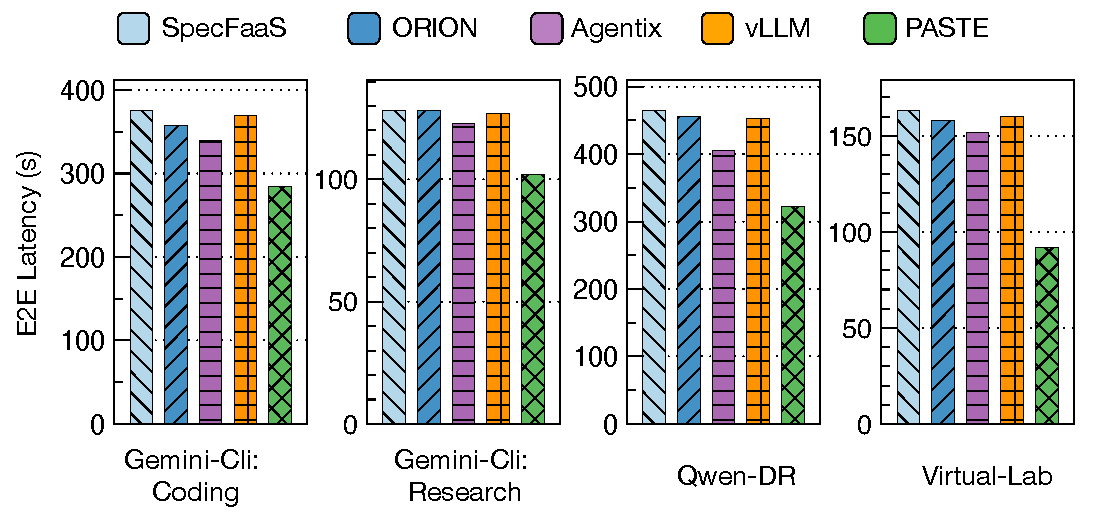
\includegraphics[width=\columnwidth]{images/ATC/E2E_overall.pdf}
  \vspace{-0.3in}
  \caption{Average E2E latency comparison against all baselines.}
  \vspace{-0.2in}
  \label{fig:eval:e2e}
\end{figure}

The improvement holds across both average and tail latency: the combination of speculative tool execution and LLM--tool co-scheduling reduces exposed tool stalls and lowers LLM-side waiting.
We further quantify this mechanism with a time breakdown in Sec~\ref{sec:eval:breakdown}.

\subsection{Tool-Side Acceleration}
\label{sec:eval:tool}

We next isolate \sys's ability to accelerate the tool side of agent execution.
Since vLLM and Agentix change the LLM-side serving policy but do not accelerate the tool execution path, this experiment compares \sys only with the two tool-side baselines, ORION and SpecFaaS.
Both baselines are backed by vLLM for LLM serving.

Figure~\ref{fig:eval:tool} reports average tool latency aggregated across all agents, and Figure~\ref{fig:eval:tool_cdf} plots the corresponding per-task CDF.
Across agents and benchmarks, \sys significantly reduces observed tool latency relative to both ORION and SpecFaaS.
\sys reduces average tool latency by up to 55.2\% and p99 tool latency by up to 60.6\%.
Aggregated across configurations, the average tool-side speedup is 1.71$\times$ over ORION and 1.83$\times$ over SpecFaaS.
These gains are consistent with speculative execution making predicted tool results available before they appear on the exposed critical path.

\begin{figure}[t]
  \centering
  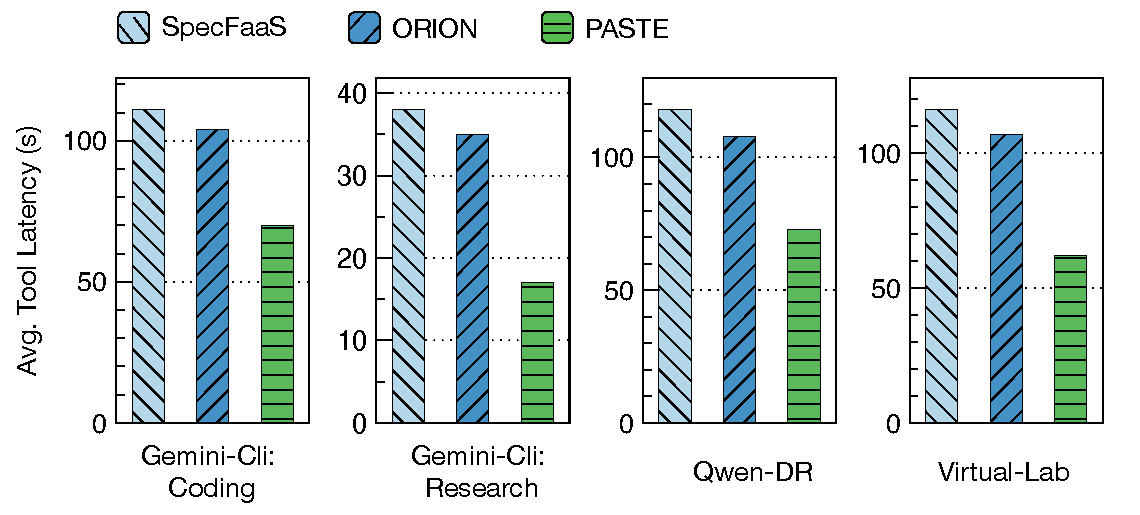
\includegraphics[width=0.9\columnwidth]{images/Evaluation/tool_overall.pdf}
  \vspace{-0.2in}
  \caption{Average tool latency comparison against tool-side baselines.}
  \label{fig:eval:tool}
  \vspace{-0.1in}
\end{figure}

\begin{figure}[t]
  \centering
  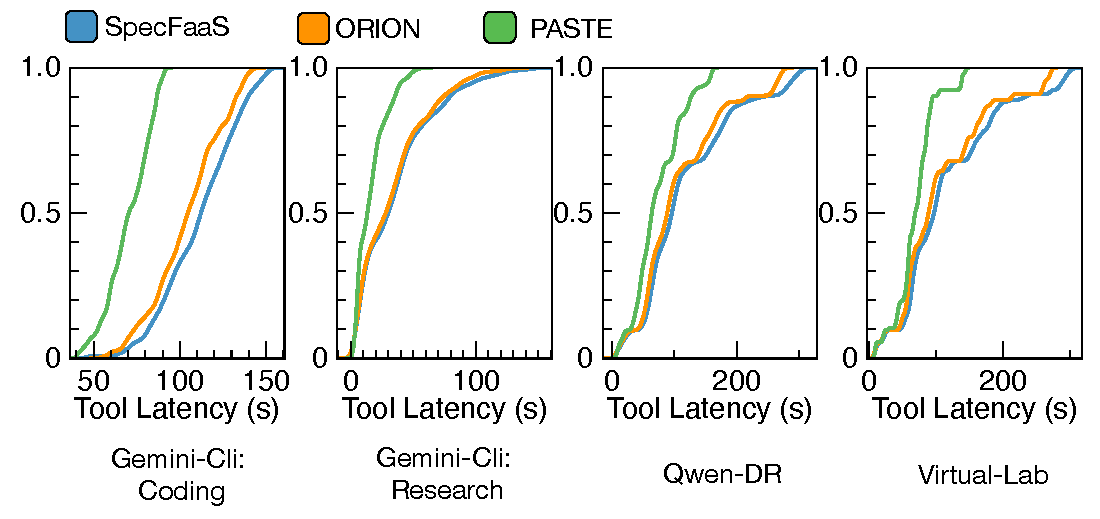
\includegraphics[width=\columnwidth]{images/Evaluation/CDF_tool_overall.pdf}
  \vspace{-0.2in}
  \caption{CDF of tool latency for each task}
  \label{fig:eval:tool_cdf}

\end{figure}





\begin{figure}[t]
  \centering
  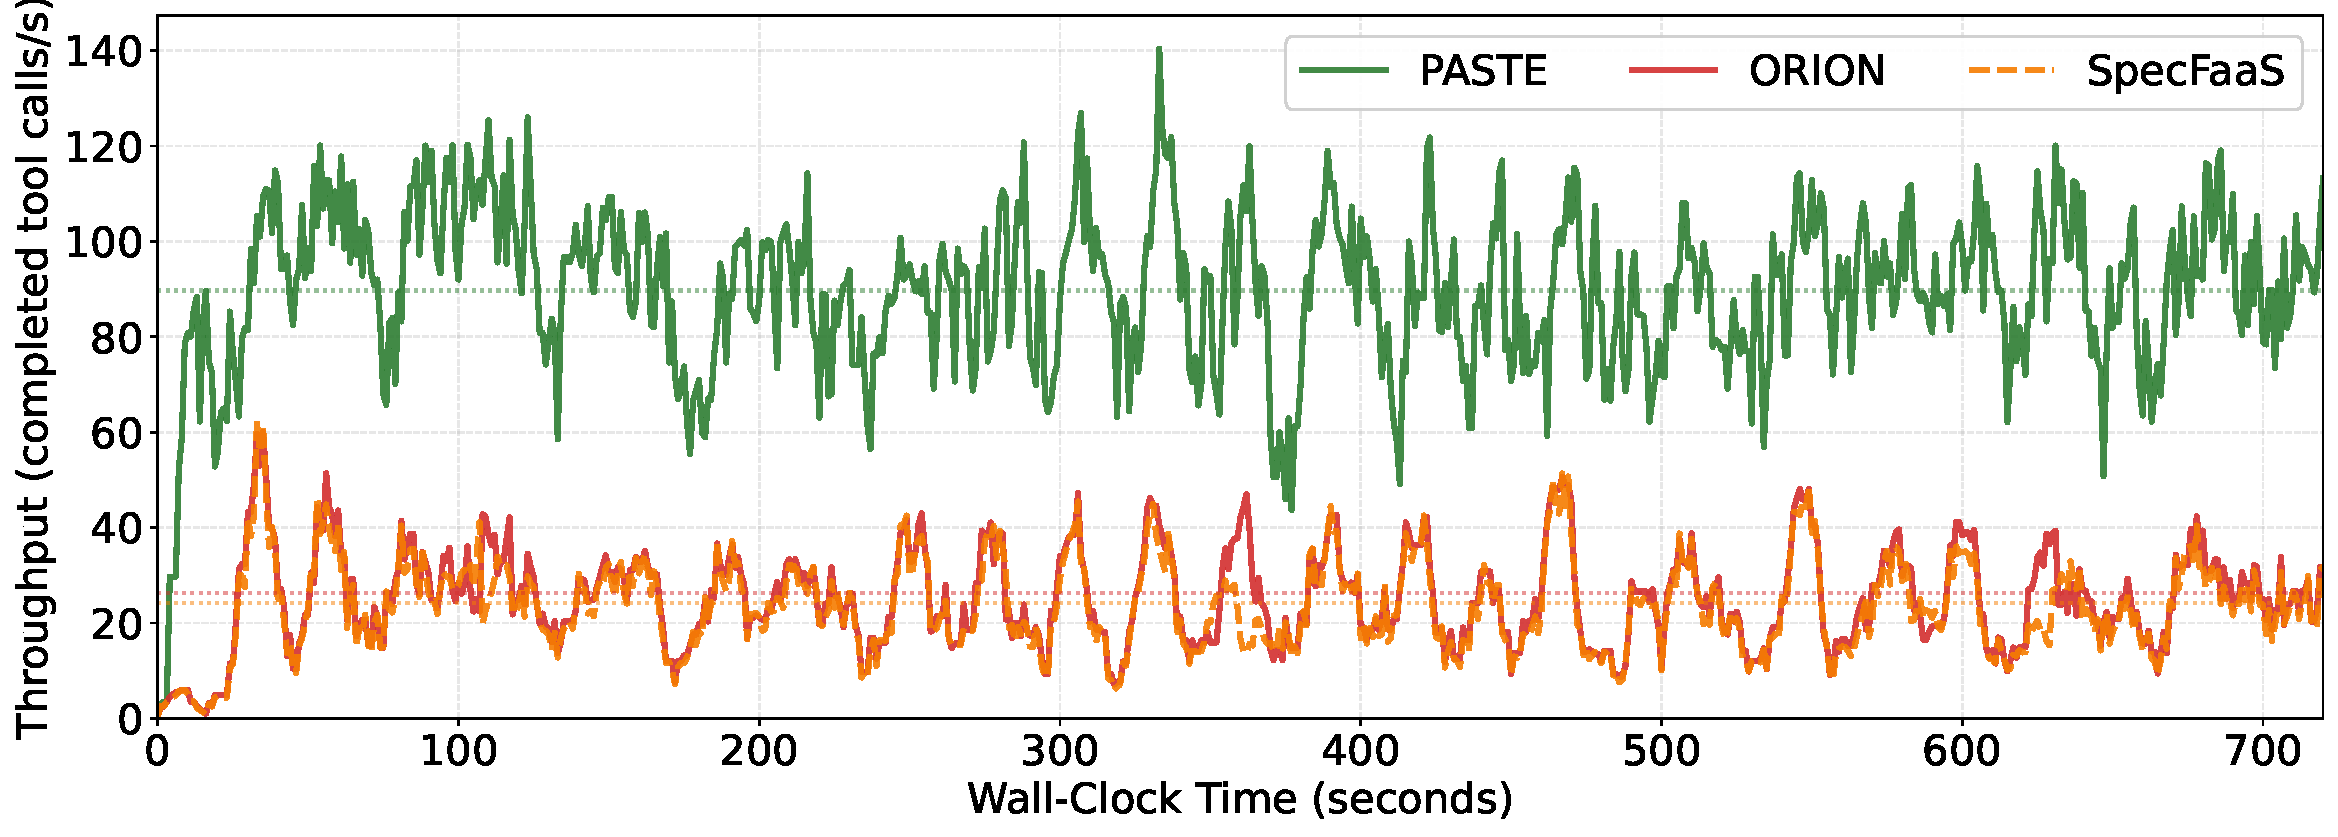
\includegraphics[width=\columnwidth]{images/Evaluation/instantaneous_throughput_timeline.pdf}
  \vspace{-0.2in}
  \caption{Tool throughput under trace-driven arrivals.}
  \label{fig:eval:throughput}
  \vspace{-0.1in}
\end{figure}


Figure~\ref{fig:eval:throughput} shows that the latency reduction translates into higher completed-tool throughput under bursty arrivals.
\sys completes more tool work under the same trace-driven arrivals, while keeping authoritative tool calls on the high-priority path.

Finally, we aggregate all tasks and examine \sys's tool-side speedup relative to the tool baselines.
Figure~\ref{fig:speedup-cdf} reports the CDF of per-request tool speedup over ORION and SpecFaaS after pooling all requests.
Most requests observe positive speedup (97\% above 1$\times$), while the worst cases remain close to parity, consistent with \sys's low speculation overhead when predictions do not hit.

\begin{figure}[t]
    \centering
    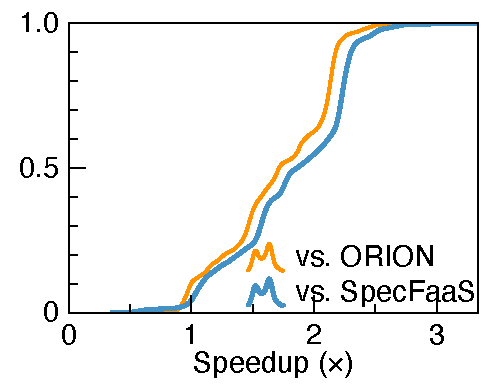
\includegraphics[width=0.45\columnwidth]{images/Evaluation/Speedup-tool-CDF.pdf}
    \vspace{-0.15in}
    \caption{CDF of per-request tool speedup over ORION/SpecFaaS.}
    \label{fig:speedup-cdf}
    \vspace{-0.2in}
\end{figure}


These gains are robust across agents, benchmarks, and LLM settings.
Improvements are largest for tool-heavy tasks where tool stalls dominate the critical path, but remain non-negative for more LLM-dominated tasks, indicating that \sys introduces low overhead when speculation does not hit.
Overall, speculative tool execution reliably converts a portion of tool-wait time into ready speculative results, improving both median and tail tool latency.


\subsection{Time Breakdown Analysis}
\label{sec:eval:breakdown}

To explain \emph{why} \sys reduces E2E latency, we instrument the runtime and attribute time to two components: the exposed tool-side path and the LLM-side serving path.
The tool-side path includes tool startup and execution time that remains visible on the task critical path, while the LLM-side path includes model execution and queueing before the next agent turn can run.

Figure~\ref{fig:eval:breakdown} reports the breakdown for vLLM, Agentix, ORION, SpecFaaS, and \sys.
\sys reduces both components rather than shifting cost between them: exposed tool-side time falls to 34~s from 84--89~s under the tool-side baselines, while the LLM-side component falls to 186~s from 226--249~s under the LLM-side baselines.
This corresponds to roughly 60\% less exposed tool time and 18\%--25\% less LLM-side time.

\begin{figure}[t]
  \centering
  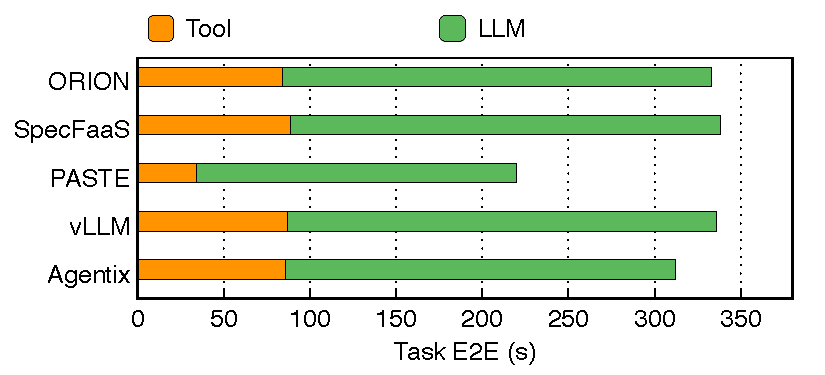
\includegraphics[width=\columnwidth]{images/Evaluation/evaluation_tool_llm.pdf}
  \vspace{-0.3in}
  \caption{Time breakdown across all baselines.}
  \label{fig:eval:breakdown}
  \vspace{-0.2in}
\end{figure}


These results confirm that \sys's speedups come from both sides of the loop.
ORION and SpecFaaS improve the tool path but leave LLM serving unchanged, while Agentix reduces LLM-side waiting but does not hide exposed tool stalls.
By combining speculative tool execution with LLM--tool co-scheduling, \sys reduces the two visible sources of latency at the same time.


\subsection{System Scalability}
\label{sec:eval:scalability}

We next evaluate scalability to determine whether \sys maintains low latency under many concurrent agent sessions, and to verify that speculation does not harm isolation by increasing queueing for authoritative tool calls.
We stress the system by sweeping arrival rate and concurrent sessions while holding resource budgets fixed.
We compare scalability against vLLM and Agentix because the multi-session bottleneck is the LLM serving engine: tool-side acceleration has limited impact as concurrency increases, while LLM queueing dominates task-level latency.

Figure~\ref{fig:eval:scalability} summarizes \sys's E2E speedup performance as workload increases.
At each concurrency, \sys sustains at least 1.27$\times$ speedup over vLLM and 1.24$\times$ over Agentix.
Pooled across the sweep, the corresponding speedups are 1.50$\times$ and 1.30$\times$.
%
These results demonstrate that \sys scales without violating isolation: speculative work is throttled by explicit budgets and remains preemptible, so it does not crowd out authoritative tool execution.

\begin{figure}[t]
  \centering
  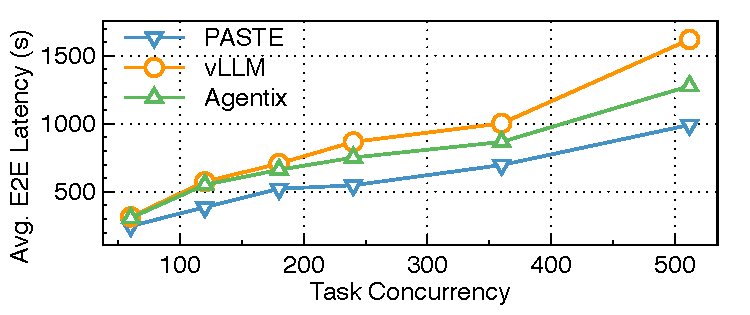
\includegraphics[width=\columnwidth]{images/Evaluation/scalability.pdf}
  \vspace{-0.3in}
  \caption{Scalability under multi-session concurrent agent requests: speedup compared with LLM-side baselines.}
  \label{fig:eval:scalability}
  \vspace{-0.1in}
\end{figure}




\subsection{Ablation Study}
\label{sec:eval:ablation}

We isolate the contribution of each scheduling component by comparing \sys with two ablated variants and two agent/LLM serving baselines.
\textbf{PASTE-Tool-Only} enables tool-side acceleration through speculative tool execution, but disables the LLM--Tool Co-Scheduler; tool-returning sessions therefore re-enter the LLM side without gain-aware pacing.
\textbf{PASTE-LLM-Only} disables speculative tool execution and only uses first-come-first-served LLM admission to reduce excessive GPU load.
We also compare against vLLM~\cite{kwon2023efficient} and Agentix~\cite{luo2025autellix}.

\begin{figure}[t]
  \centering
  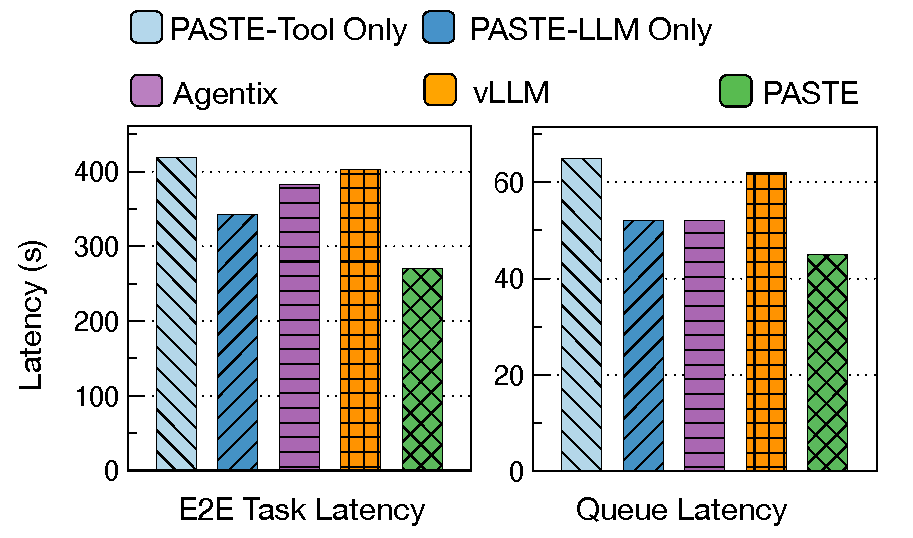
\includegraphics[width=0.9\columnwidth]{images/ATC/ablation.pdf}
  \vspace{-0.1in}
  \caption{Task's E2E latency in ablation evaluation.}
  \label{fig:eval:ablation}
  \vspace{-0.1in}
\end{figure}

Figure~\ref{fig:eval:ablation} shows that both sides are necessary.
PASTE-Tool-Only performs worst: although tool speculation shortens tool execution, it also makes sessions return to the LLM more frequently and in tighter bursts, increasing average LLM queueing time to 65~s and raising E2E latency to 419~s.
PASTE-LLM-Only reduces queueing pressure, but without speculative tools it cannot hide exposed tool time, so E2E latency remains 342~s.
Full \sys combines the two mechanisms: speculative tools reduce exposed tool stalls, while LLM--tool co-scheduling preserves this gain before it turns into GPU queueing.
As a result, \sys reduces E2E latency to 270~s and LLM queueing time to 45~s, cutting E2E latency by 21.1\%--35.6\% and queueing time by 13.5\%--30.8\% across the ablations and serving baselines.


\subsection{Pattern Prediction Accuracy}
\label{sec:eval:accuracy}




Speculative execution is only effective when the system can correctly anticipate near-future tool calls.
We therefore measure prediction quality using \textbf{Top-1 accuracy} (the highest-probability predicted tool matches the next tool actually invoked) and \textbf{Top-3 recall} (the next tool appears among the three most likely predictions).
Top-3 recall is particularly relevant because \sys may speculatively execute multiple candidates within a bounded budget.
We also report \textbf{overall hit rate}, defined per tool call as the probability that \emph{any} speculatively executed prediction matches the next tool actually invoked.
Because \sys can issue multiple predictions (and increase the number of candidates when the system is lightly loaded and spare resources are available), overall hit rate can be high even when Top-1 accuracy is low.

Figure~\ref{fig:eval:accuracy} reports prediction quality by benchmark family.
Overall, the predictor achieves up to 27.8\% Top-1 accuracy, 43.9\% Top-3 recall, and 93.8\% overall hit rate.
Accuracy is higher for structured tool sequences (e.g., compilation/test loops) and lower for open-ended exploration patterns typical of broad research tasks.


Despite imperfect Top-1 accuracy, strong Top-3 recall is sufficient in practice: \sys can speculate on a small set of likely tools and still reduce exposed tool time when any candidate hits.
When prediction is uncertain, the explicit speculation budget bounds wasted work and prevents negative interference with authoritative execution.



\subsection{Side-effect Evaluation}
\label{sec:eval:sideeffects}

Finally, we evaluate safety to ensure that enabling speculation does not change externally visible behavior or violate isolation, even under mispredictions.
We audit speculative executions to measure (i) how many speculative actions would have caused external side effects, (ii) whether such effects were prevented from committing, and (iii) any divergences in final outputs relative to authoritative-only execution.
%
Across all workloads, \sys detects 602 potentially side-effecting speculative actions among over 20,000 speculative actions and prevents them from committing. No task produces a different final result compared with the baselines.
%
Overall, the results support \sys's safety claim: speculative actions are contained by policy and sandboxing and only become externally visible after authoritative confirmation.

\begin{figure}[t]
  \centering
  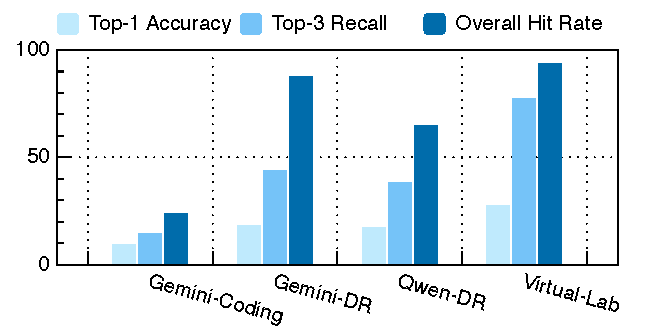
\includegraphics[width=0.85\columnwidth]{images/Evaluation/predict.pdf}
  \vspace{-0.1in}
  \caption{Pattern prediction quality: Top-1 accuracy, Top-3 recall, and overall hit rate.}
  \vspace{-0.1in}
  \label{fig:eval:accuracy}
\end{figure}

\subsection{Resource Overhead}
\label{sec:eval:efficiency}

Resource overhead remains small relative to the latency savings.
At a moderate speculation budget, \sys reduces tool execution latency by 48\% using 1--3 otherwise idle CPU cores and 250 MB of additional memory.
Normalized by latency saved, this costs 0.02 core-seconds of CPU, 2.6 MB of memory, and 0.9 MB of network bandwidth per second of latency reduction.
These results show that \sys can be tuned to a practical ``sweet spot'' in which most speculative work is converted into useful latency reduction, while the remaining waste is bounded by explicit budgets.
Overall, PASTE is lightweight enough to be deployed as a sidecar alongside existing agent runtimes, delivering latency wins without requiring dedicated infrastructure or disruptive changes to the execution stack.
%
The pattern predictor and scheduling policy add less than 100 ms of latency overhead.
